\section{Systemmodelle}
\subsection{Anwendungsfälle}
\subsection{Bedienung der Android App}
\begin{center}
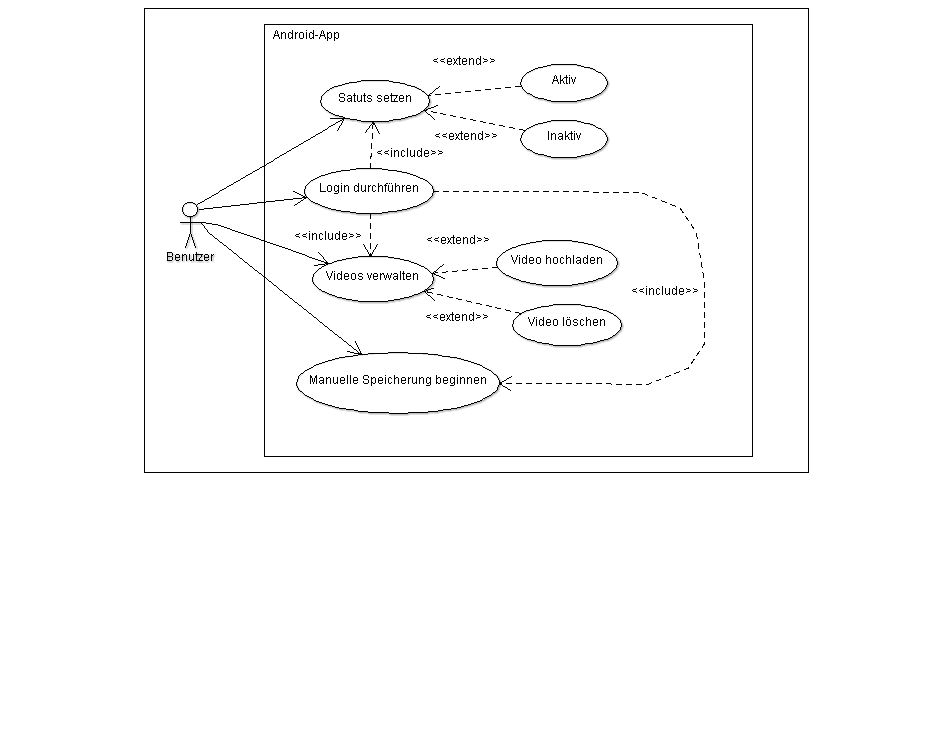
\includegraphics[width=1\textwidth]{subtopicsFuncspec/systemModels/AppAWFDiagram.png}
\end{center}
Dieser Anwendungsfall beschreibt die Bedienung der App. 
Der Benutzer kann hierbei mehrere Aktionen ausführen:
\begin{description}
\item Login durchführen
\item Videos verwalten
\item Den Status setzen
\item Manuelle Speicherung beginnen
\end{description}
Um auf alle Funktionen zugreifen zu können muss sich der Benutzer zunächst auf der App einloggen. 
Wenn der Benutzer sein aufgenommenes Videomaterial verwalten will kann er zum einen die Videos auf den Web-Service hochladen oder die Videos löschen.
Des weiteren kann er den Status der „Aufnahme“ auf aktiv/inaktiv setzen. Bei aktiv ist der Ringpuffer angeschaltet. 
Außerdem kann man einen manuellen Speichervorgang ohne des Auslösen des Sensors beginnen um zum Beispiel.

\subsection{Bedienung der Website}
\begin{center}
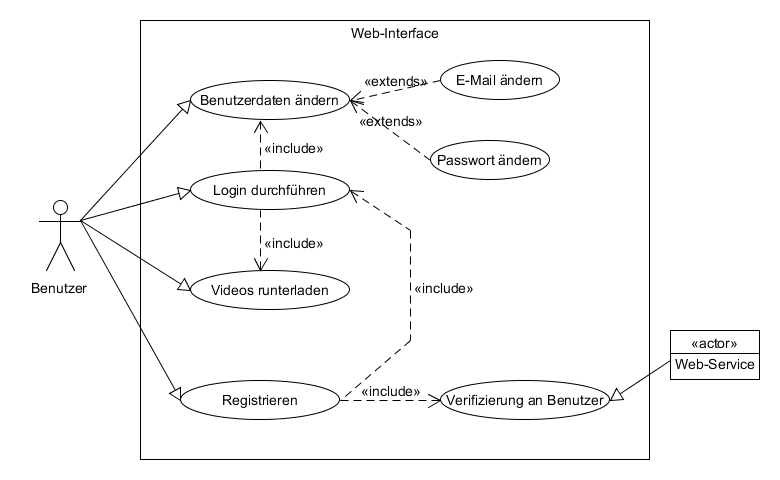
\includegraphics[width=1\textwidth]{subtopicsFuncspec/systemModels/WebsiteAWFDiagram.png}
\end{center}
Dieser Anwendungsfall beschreibt die Bedienung der Website.
Der Benutzer kann hierbei mehrere Aktionen ausführen:
\begin{description}
\item Login durchführen
\item Registrieren
\item Benutzerdaten ändern
\item Videos runterladen
\end{description}
Um den Service der App und der Website zu nutzen muss sich der Benutzer zu Beginn mit seinen Benutzerdaten registrieren. 
Nun kann er den Login auf der Website oder App durchführen um die Funktionen beider Applikationen zu nutzen. 
Ist der Benutzer eingeloggt kann er seine Benutzerdaten ändern und bereits hochgeladene Videos nach der Anonymisierung runterladen.
Nach der Registrierung und Änderung von Benutzerdaten schickt der Web-Service eine Verifizierungsmail an den Benutzer.